\section{Customer guide} \label{_cliente}
\subsection{Purpose of the section}
The goal of this section of the document is to describe what a customer can do using EmporioLambda.

\subsection{How to land to the web-application} \label{_homepage}
The only current way to access the application is by direct link. After accessing the the application by link you will land to the homepage.

\subsection{How to Sign in} \label{_signin}
In order to login in the platform you have to pressing the login button from any page of the e-commerce.
\begin{figure}[H]
    \centering
    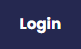
\includegraphics[width=5em]{res/images/cliente/loginbutton.png}
    \caption{Sign in}
\end{figure}

Remember: if you don't have an account you can always register one following the \hyperref[_signup]{instructions}.
To successfully login please submit the following info: 

\begin{itemize} 
    \item \textbf{Email};
    \item \textbf{Password}.
\end{itemize}

\begin{figure}[H]
    \centering
    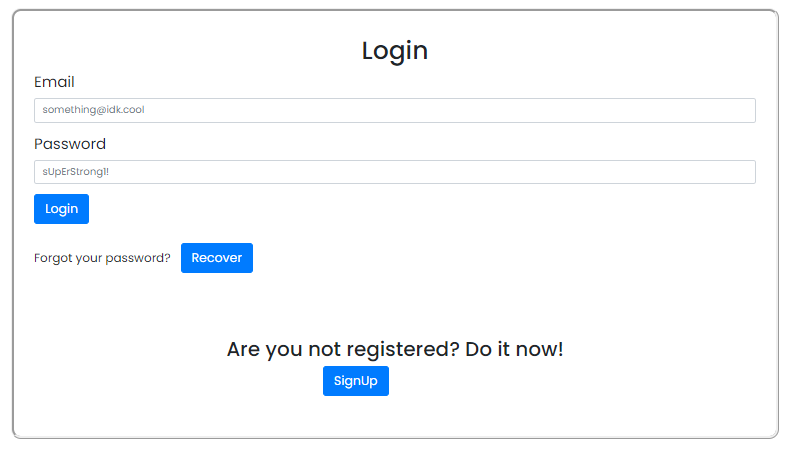
\includegraphics[width=30em]{res/images/cliente/signin.png}
    \caption{Sign in}
\end{figure}

\subsection{How to Sign up} \label{_signup}
In order to create a new account you have to press the SignUp button. To successfully register a new you have to submit the following info:
\begin{itemize} 
    \item \textbf{Email};
    \item \textbf{Password};
    \item \textbf{Name};
    \item \textbf{Surname}.
\end{itemize}
To ensure the user to write the email and the password correctly, the application force to re-enter these data twice.

\begin{figure}[H]
    \centering
    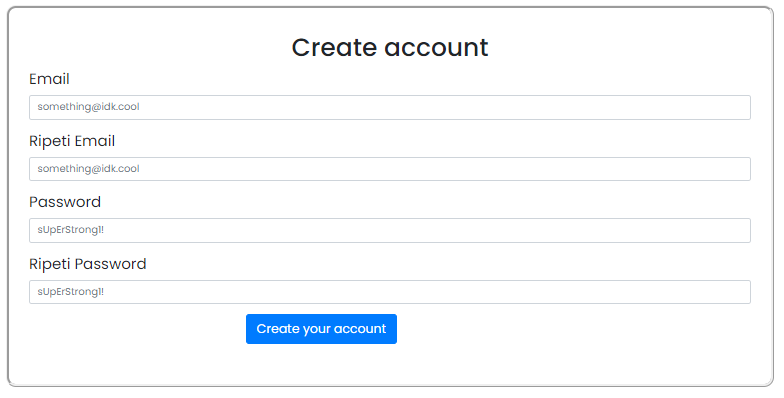
\includegraphics[width=30em]{res/images/cliente/signup.png}
    \caption{Sign up}
\end{figure}

After that you will receive an e-mail with the code to insert to verify the account.

\begin{figure}[H]
    \centering
    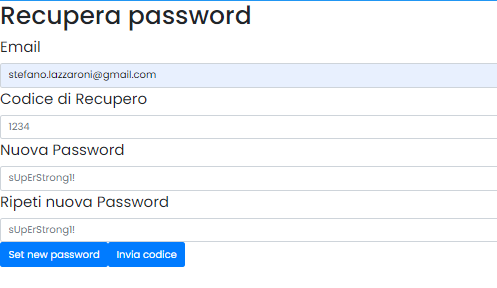
\includegraphics[width=30em]{res/images/cliente/verify.png}
    \caption{Verify code}
\end{figure}


\subsection{How to Sign out} \label{_signout}
In order to be able to sign out you have to be signed in. Then you will find the logout button in the Navigation Bar (Top right).

\begin{figure}[H]
    \centering
    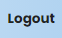
\includegraphics[width=5em]{res/images/cliente/signout.png}
    \caption{Sign out}
\end{figure}

\subsection{How to restore your password} \label{_passwordrecover}
To restore your password, in the \hyperref[_signup]{sign up page}, you find the recover password button.
\begin{figure}[H]
    \centering
    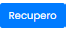
\includegraphics[width=5em]{res/images/cliente/recover.png}
    \caption{Recover button}
\end{figure}

Then you will be asked to insert the e-mail of the account you want to log in into.
\begin{figure}[H]
    \centering
    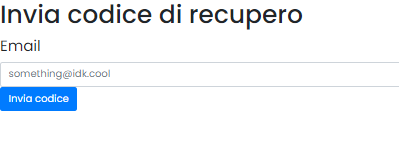
\includegraphics[width=30em]{res/images/cliente/recoveremail.png}
    \caption{Code field}
\end{figure}

You will receive an e-mail with a code. Insert it and set the new password.
\begin{figure}[H]
    \centering
    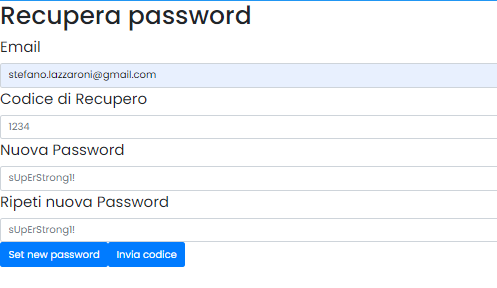
\includegraphics[width=30em]{res/images/cliente/newpassword.png}
    \caption{New password fields}
\end{figure}


\subsection{How to look for a product} \label{_lookforproduct}
There are several ways to find a product in the website. One way is to find the desired product in the \textbf{Best products} section that is in the \hyperref[_homepage]{homepage}. Another way is to be in a Product Listing Page. You can reach this page by:
\begin{itemize} 
    \item \textbf{Typing in the search bar};
    \item \textbf{Clicking the category name}.
\end{itemize}

\begin{figure}[H]
    \centering
    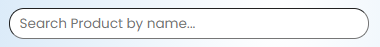
\includegraphics[width=22em]{res/images/cliente/searchingbar.png}
    \caption{Searching Bar}
\end{figure}

\begin{figure}[H]
    \centering
    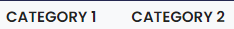
\includegraphics[width=18em]{res/images/cliente/categories.png}
    \caption{Categories}
\end{figure}

\begin{figure}[H]
    \centering
    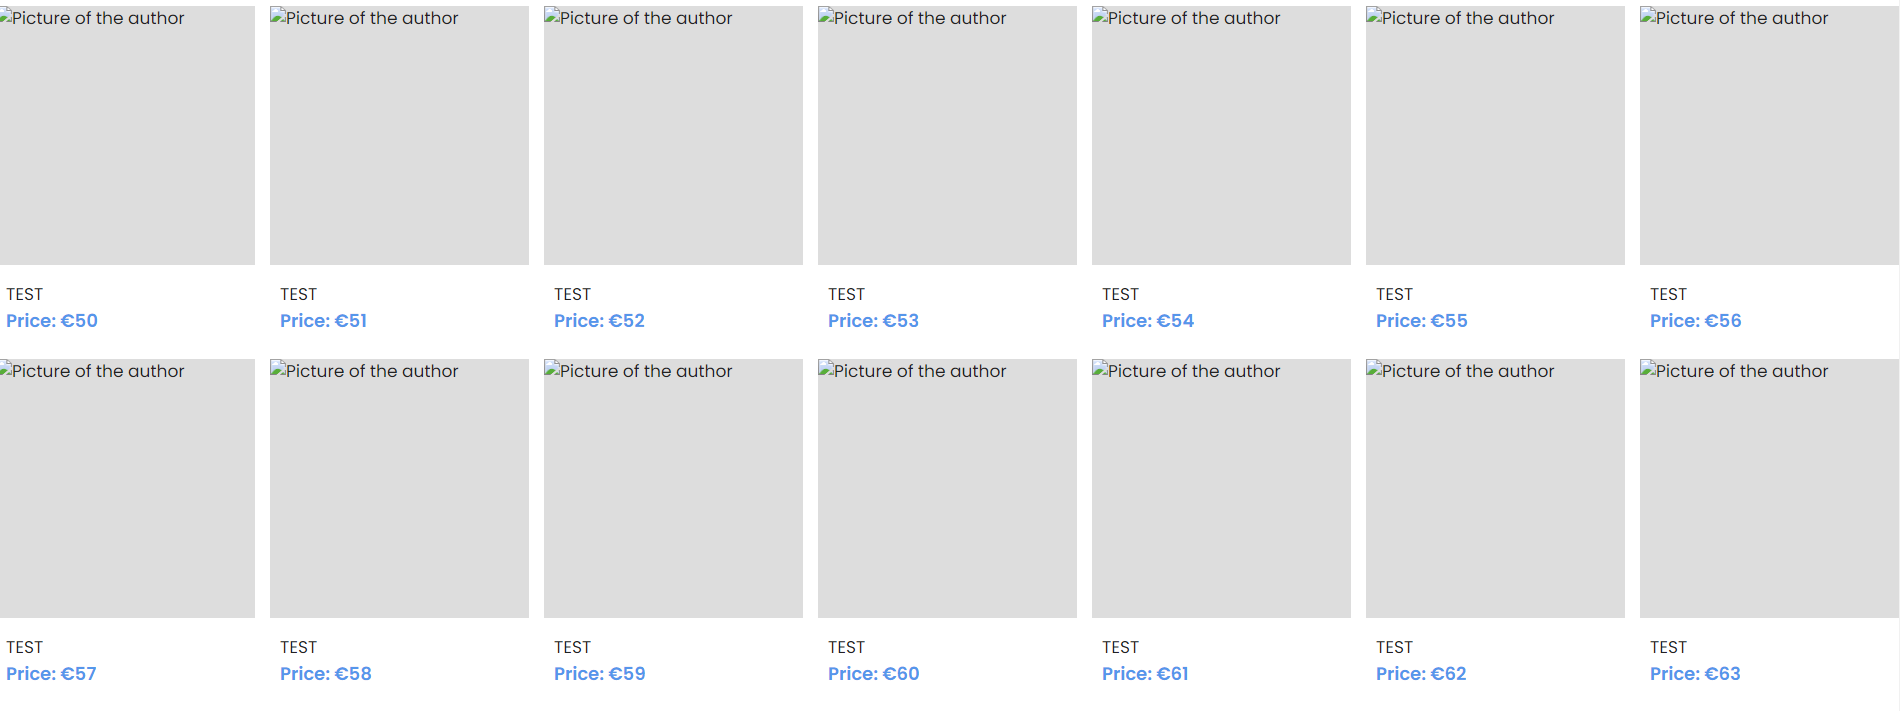
\includegraphics[width=\linewidth]{res/images/cliente/plp.png}
    \caption{Product Listing Page}
\end{figure}

\subsubsection{How to refine your search list}
There are 2 more options to find the best product for you:
\begin{enumerate} 
    \item \textbf{Filter between costs}: it allows to filter the list of products between 2 costs (minimum and maximum);
    \item \textbf{Order by cost}: it allows to order the list from the cheapest to the more expensive and vice versa.
\end{enumerate}

\begin{figure}[H]
    \centering
    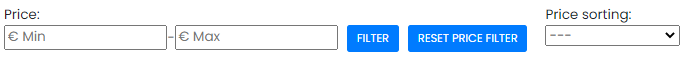
\includegraphics[width=35
    em]{res/images/cliente/refinementtools.png}
    \caption{Refinement tools}
\end{figure}

\subsection{How to buy a product} \label{_buyproduct}
In order to buy a product, you have to follow these steps:
\begin{itemize} 
    \item \textbf{Find the desired product}: this action can be done via these \hyperref[_lookforproduct]{instructions};
    \item \textbf{Add the product to the cart}: this action can be done via these \hyperref[_addproduct]{instructions};
    \item \textbf{Check the cart}: this action can be done via these \hyperref[_checkcart]{instructions};
    \item \textbf{Proceed to the checkout}: this action can be done via these \hyperref[_checkout]{instructions}.  
\end{itemize}

\subsubsection{How to add a product to the cart} \label{_addproduct}
In order to add a product to your cart first you have to find the desired product/s. You can find here the \hyperref[_lookforproduct]{instructions}.
Open the details page by clicking the desired product.
\begin{figure}[H]
    \centering
    
\includegraphics[width=40em]{res/images/cliente/pdp.png}
    \caption{Details page of product}
\end{figure}
Then you just simply select the number of items, using the + or - buttons. Then click the "Add to cart" button.
\begin{figure}[H]
    \centering
    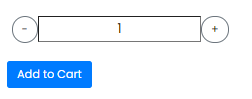
\includegraphics[width=10em]{res/images/cliente/addtocart.png}
    \caption{Add to cart}
\end{figure}

\subsubsection{How to check your cart} \label{_checkcart}
To check your cart you can simply press the cart icon in the top right corner of the page.
\begin{figure}[H]
    \centering
    
\includegraphics[width=5em]{res/images/cliente/carticon.png}
    \caption{Cart Icon}
\end{figure}
Here you can check your cart. If the cart is fine, you can proceed to the checkout by pressing the checkout button.
\begin{figure}[H]
    \centering
    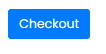
\includegraphics[width=7em]{res/images/cliente/checkoutbutton.png}
    \caption{Checkout Button}
\end{figure}

\subsubsection{How to proceed to the checkout} \label{_checkout}
In this page you have to insert all the info about billing and shipping addresses and payment method.
You can manually type  all the billing and shipping info or just use a previously stored address.
Remember: if you are typing by hand the info, you can always automatically copy the billing info into the shipping info by pressing the "Autofill with Billing Data".
\begin{figure}[H]
    \centering
    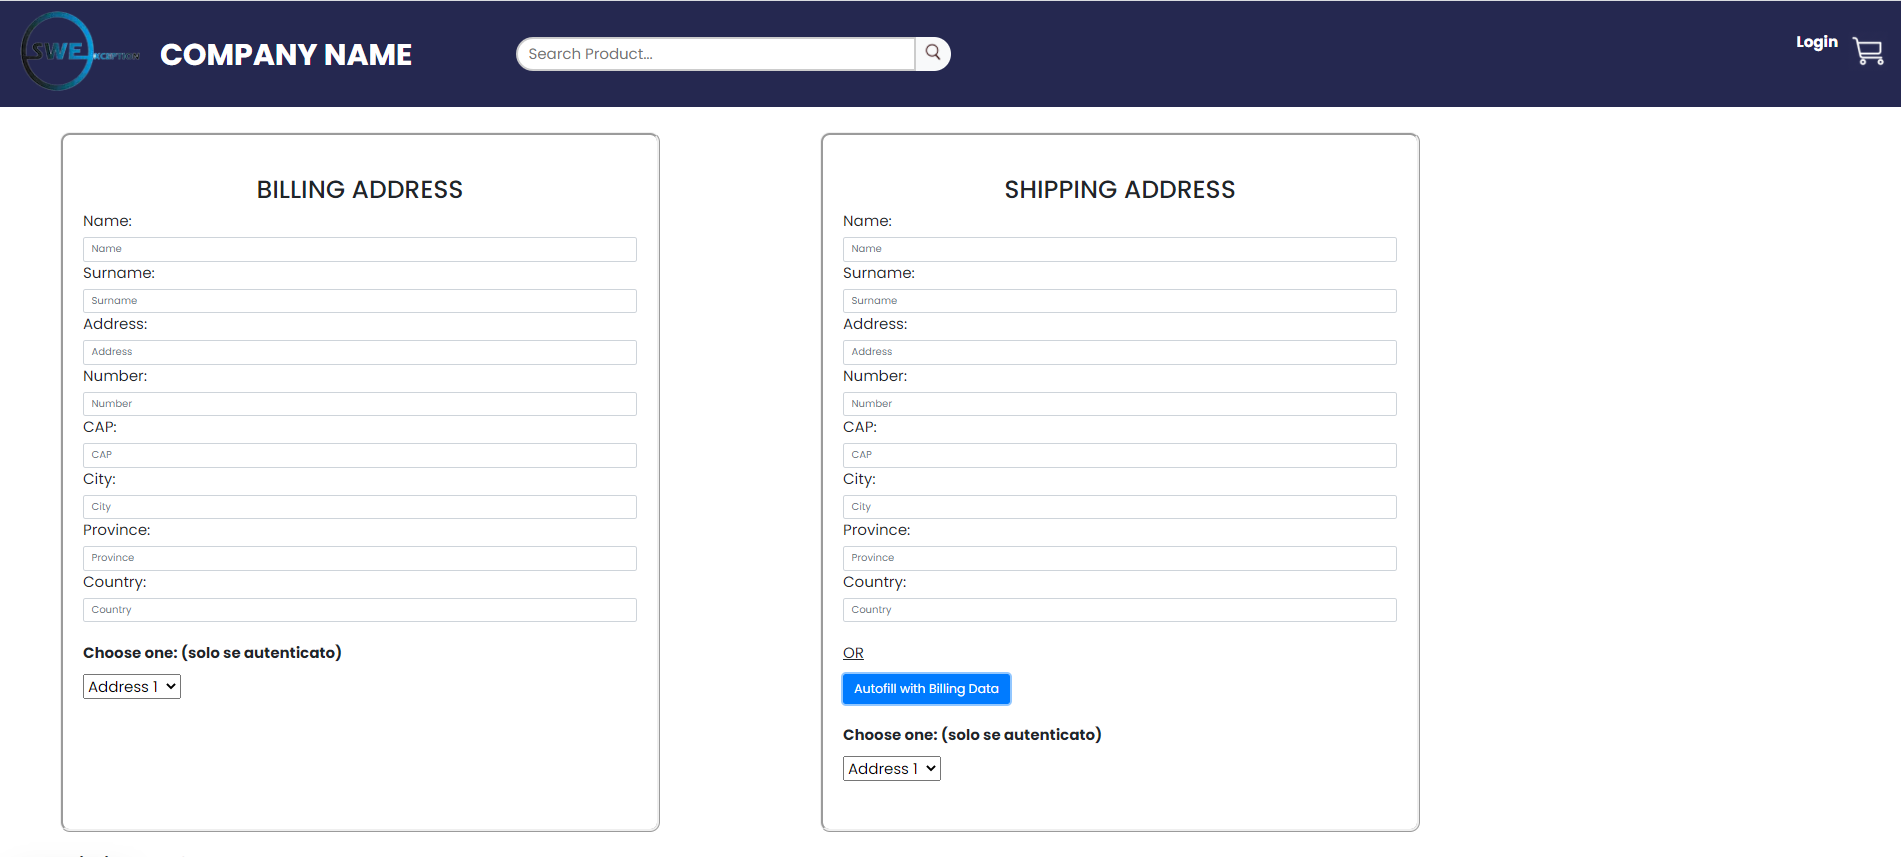
\includegraphics[width=\linewidth]{res/images/cliente/checkout.png}
    \caption{Checkout}
\end{figure}
Once you have filled all the field about billing and shipping, you have to insert the info about your credit card.
Remember: this platform will never handle payment data. Your data are securely used only by \href{https://stripe.com}{Stripe}.
\begin{figure}[H]
    \centering
    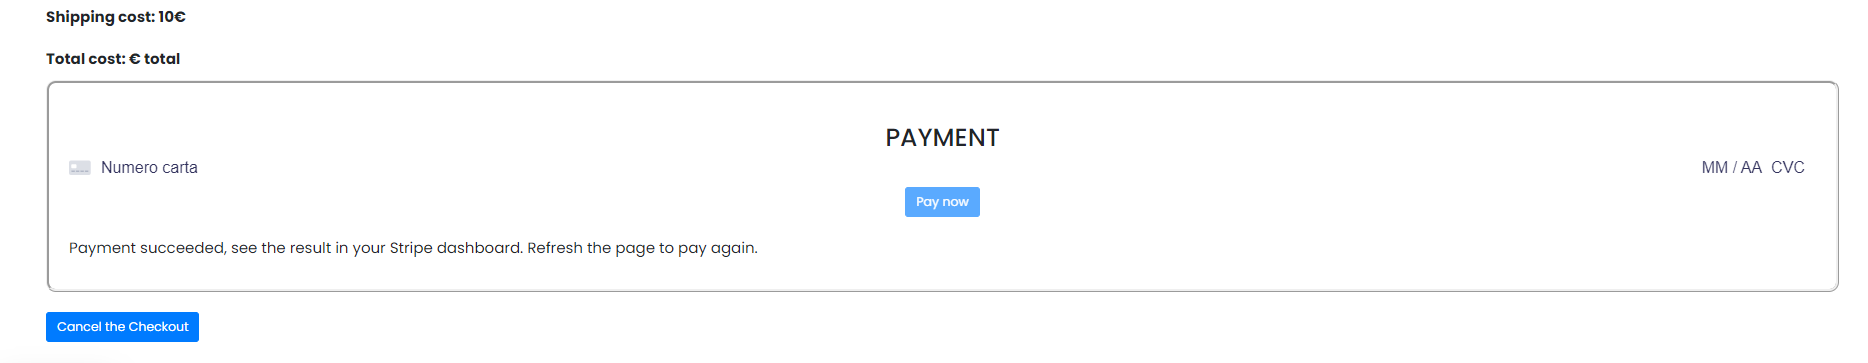
\includegraphics[width=\linewidth]{res/images/cliente/payment.png}
    \caption{Payment}
\end{figure}

\subsection{How to manage your cart} \label{_cart}
In order to manage your cart you have to access to it. This action can be done via these \hyperref[_checkcart]{instructions}.
Here you can:
\begin{itemize} 
    \item \textbf{Edit item quantity}: by pressing the + or - buttons;
    \item \textbf{Remove completely the product}: by pressing the X button of the no more desired product;
    \item \textbf{Remove completely all products}: by pressing the Remove all button;  
\end{itemize}
\begin{figure}[H]
    \centering
    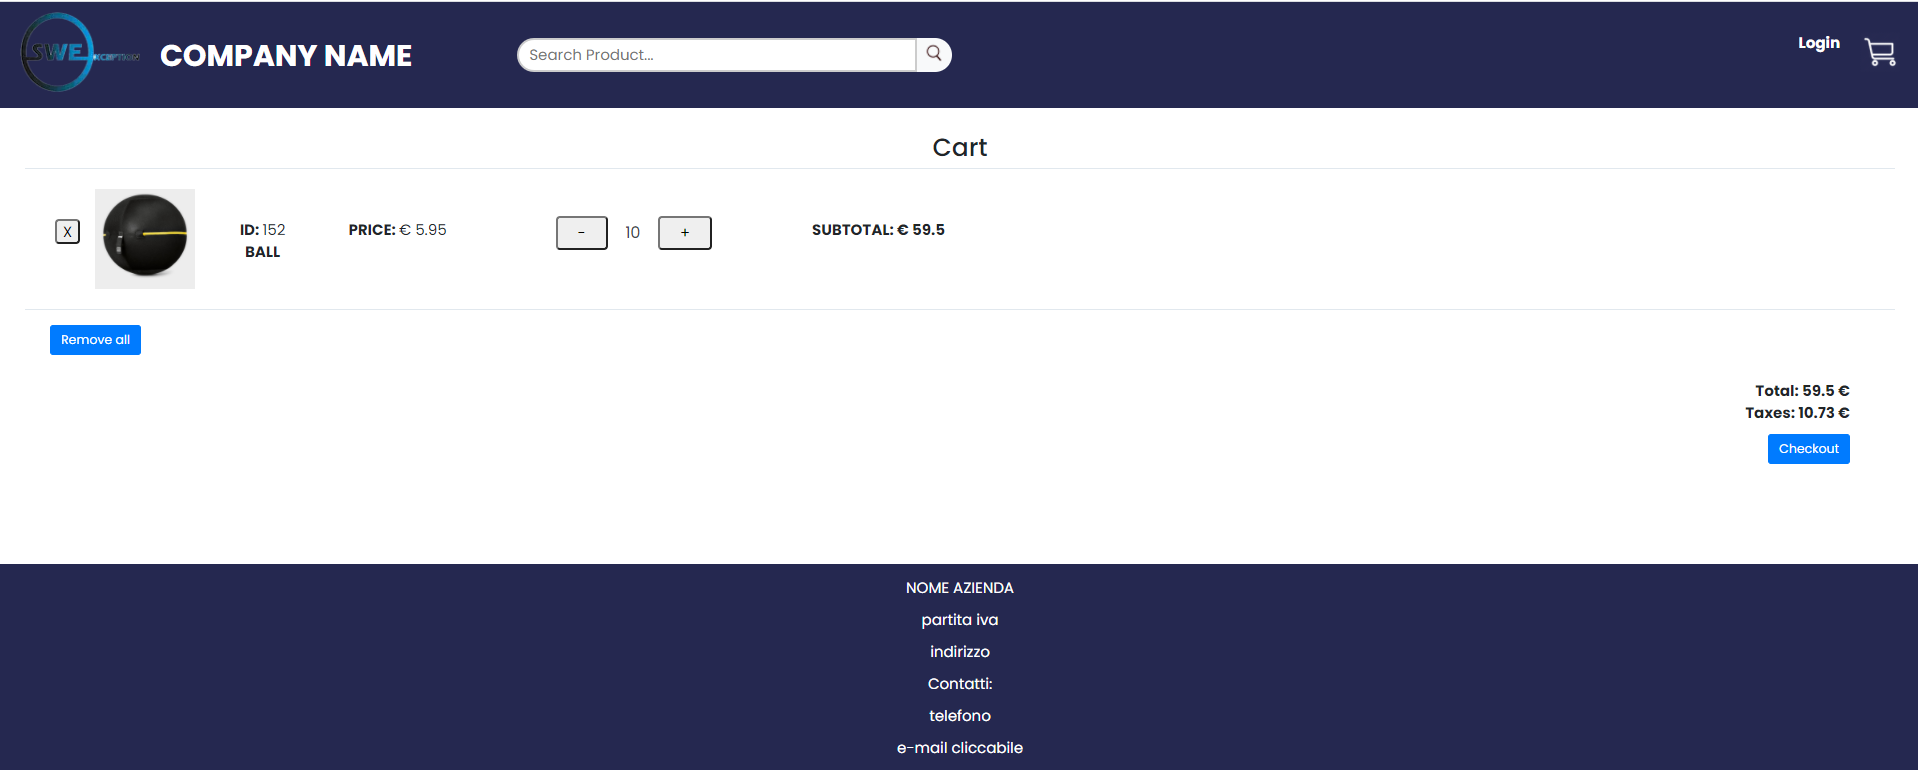
\includegraphics[width=\linewidth]{res/images/cliente/cart.png}
    \caption{Cart}
\end{figure}

\subsection{How to manage your addresses} \label{_addresses}
In order to manage your cart you have to be signed in. This action can be done via these \hyperref[_signin]{instructions}.
Then you have to access the profile page by clicking the profile button.
\begin{figure}[H]
    \centering
    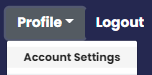
\includegraphics[width=10em]{res/images/cliente/profileaccount.png}
    \caption{Profile Button - Account settings}
\end{figure}

Here you can add a new address by filling the fields or just deleting an existing address. 
\begin{figure}[H]
    \centering
    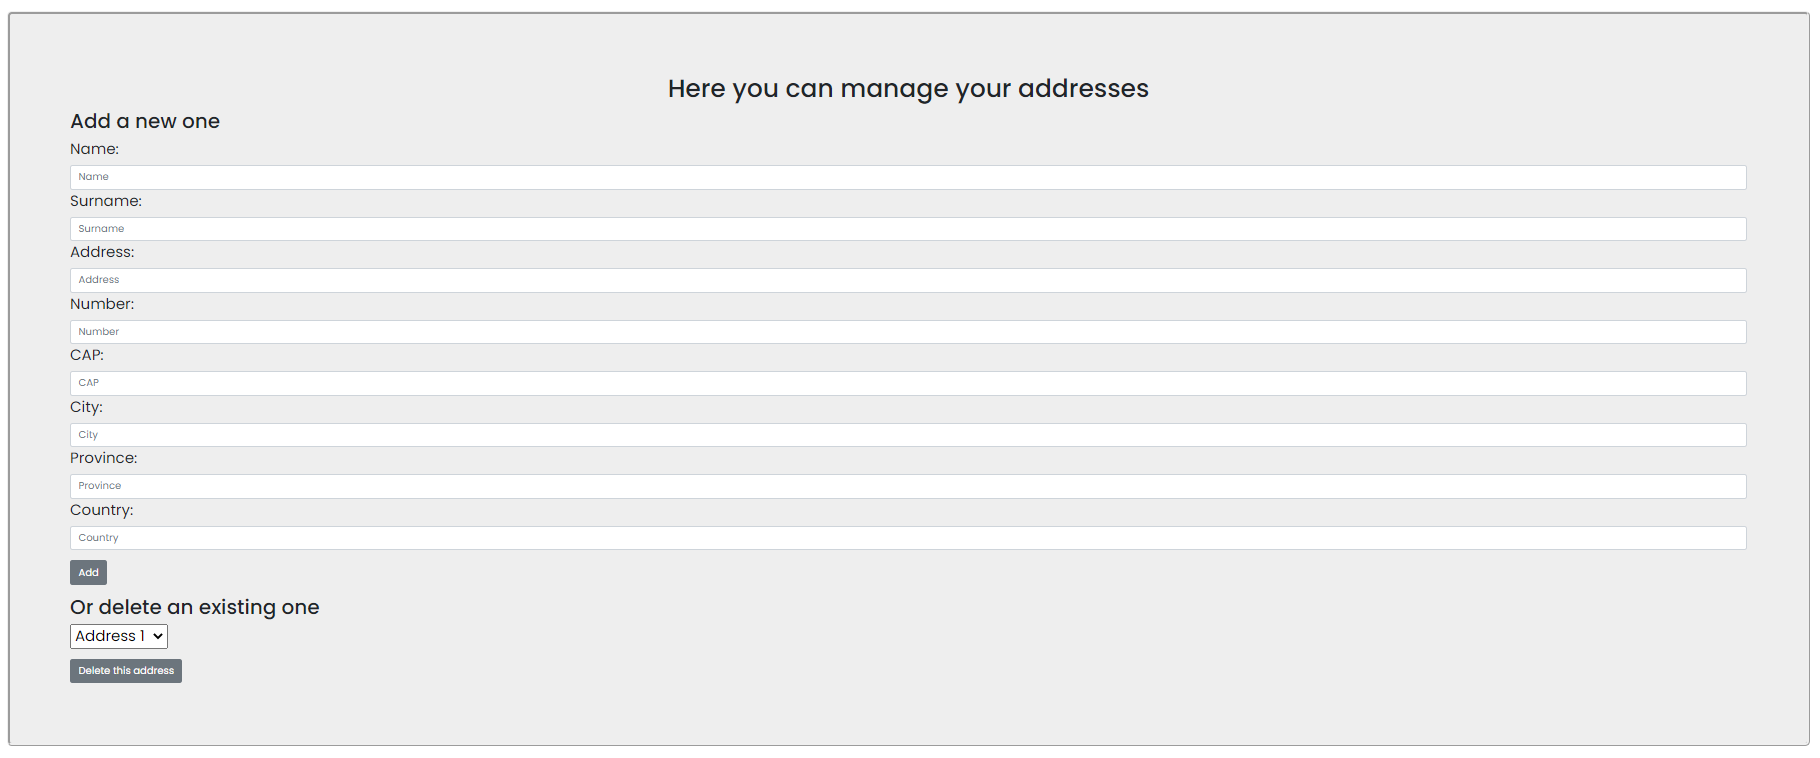
\includegraphics[width=\linewidth]{res/images/cliente/address.png}
    \caption{Address}
\end{figure}
\subsection{How to manage your orders} \label{_orders}
In order to be able to see your orders you have to be signed in. This action can be done via these \hyperref[_signin]{instructions}.
To manage your orders you have to go to click on the button of the profile and select "My orders".
\begin{figure}[H]
    \centering
    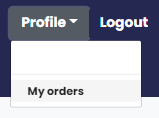
\includegraphics[width=10em]{res/images/cliente/profileorder.png}
    \caption{Profile button - My orders}
\end{figure}
Here you will find the list of your past orders.
\begin{figure}[H]
    \centering
    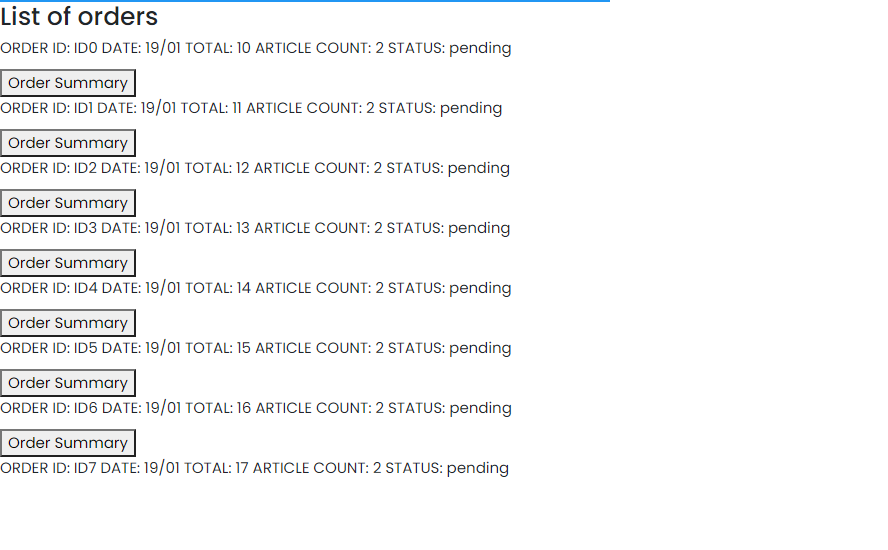
\includegraphics[width=\linewidth]{res/images/cliente/orders.png}
    \caption{Orders list}
\end{figure}
Each order has a detail page where you can:
\begin{itemize} 
    \item \textbf{Check all the info about the selected order};
    \item \textbf{Ask assistance for the order}; 
    \item \textbf{Ask to return a product of the order}; 
    \item \textbf{Ask to cancel the order}.
\end{itemize}
The last 3 options are implemented via e-mail. This allows you to directly message with the seller.
\begin{figure}[H]
    \centering
    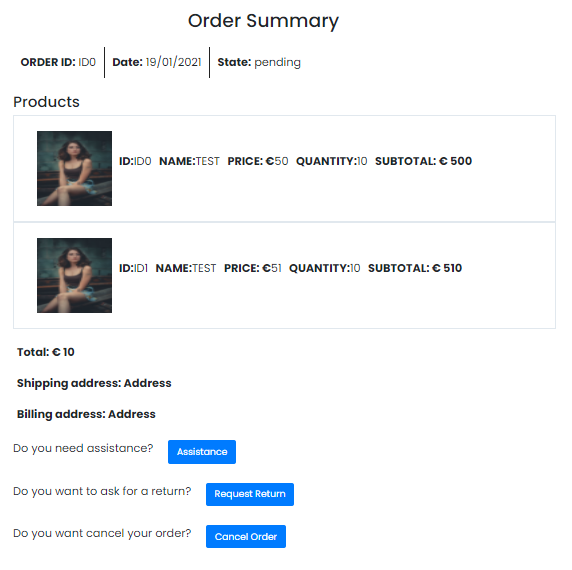
\includegraphics[width=30em]{res/images/cliente/order.png}
    \caption{Order detail}
\end{figure}

\subsection{How to manage your credentials} \label{_credentials}
In order to be able to manage your credentials you have to be signed in. This action can be done via these \hyperref[_signin]{instructions}.
Then you have to access the profile page by clicking the profile button.
\begin{figure}[H]
    \centering
    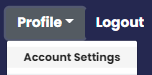
\includegraphics[width=10em]{res/images/cliente/profileaccount.png}
    \caption{Profile Button}
\end{figure}

Here you can edit your current password and your current e-mail.
To edit the password:
\begin{itemize} 
    \item \textbf{Old password}: insert the old password;
    \item \textbf{New password}: insert the new password; 
    \item \textbf{Confirm new password}: re-insert the new password. This step ensures the user not to  mistype the password.
\end{itemize}

To edit the e-mail:
\begin{itemize} 
    \item \textbf{New password}: insert the new e-mail; 
    \item \textbf{Confirm new password}: re-insert the new e-mail. This step ensures the user not to  mistype the e-mail.
\end{itemize}

\begin{figure}[H]
    \centering
    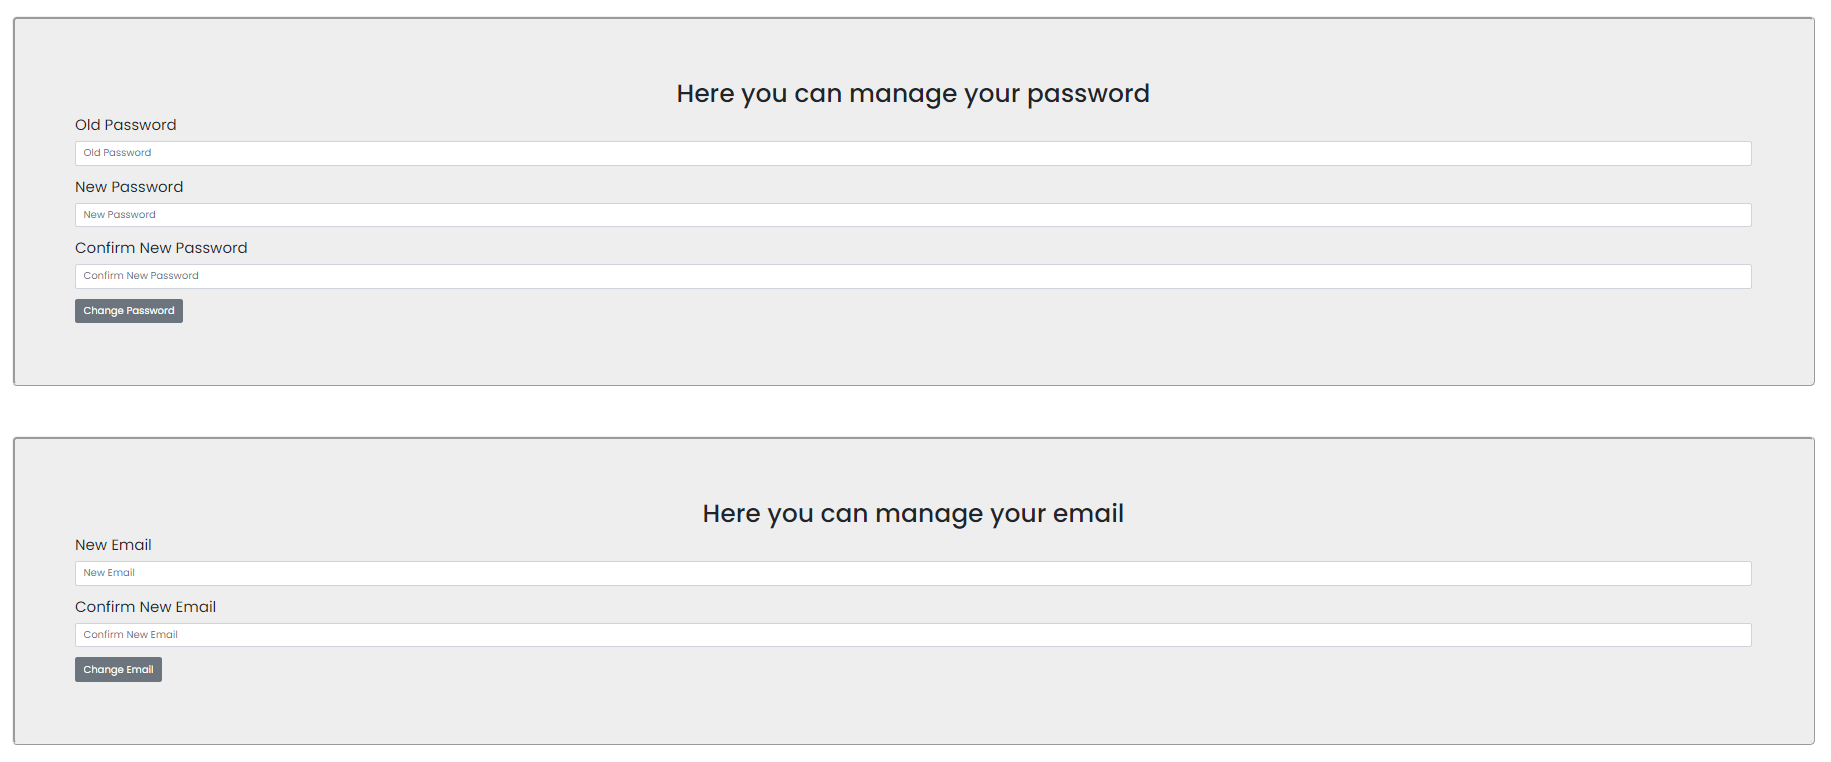
\includegraphics[width=\linewidth]{res/images/cliente/credentials.png}
    \caption{Credentials}
\end{figure}
\subsection{How to delete your account} \label{_delete}
In order to be able to request an account deletion you have to be signed in. This action can be done via these \hyperref[_signin]{instructions}.
Then you have to access the profile page by clicking the profile button.
When you click the "Request account deletion" button, you will be sending a e-mail to the seller asking to delete the account from the platform.
\begin{figure}[H]
    \centering
    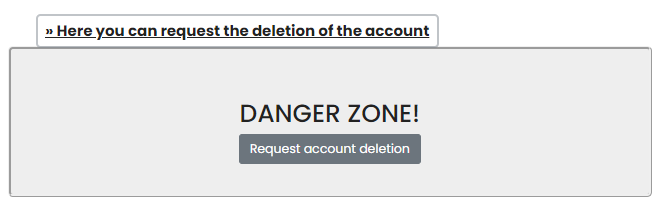
\includegraphics[width=30em]{res/images/cliente/delete.png}
    \caption{Delete Account Request}
\end{figure}

\subsection{How to contact the seller} \label{_contacts}
To contact the seller you can find the link of the e-mail in the footer of the \hyperref[_homepage]{homepage}.

